\hypertarget{part-3-image-1}{%
	\section{Part 3, Image 2}\label{part-1-design-4}}


\centering


\hypertarget{description}{%
	\subsubsection{Description}\label{description}}

\begin{description}
	\item[Image:]
	\item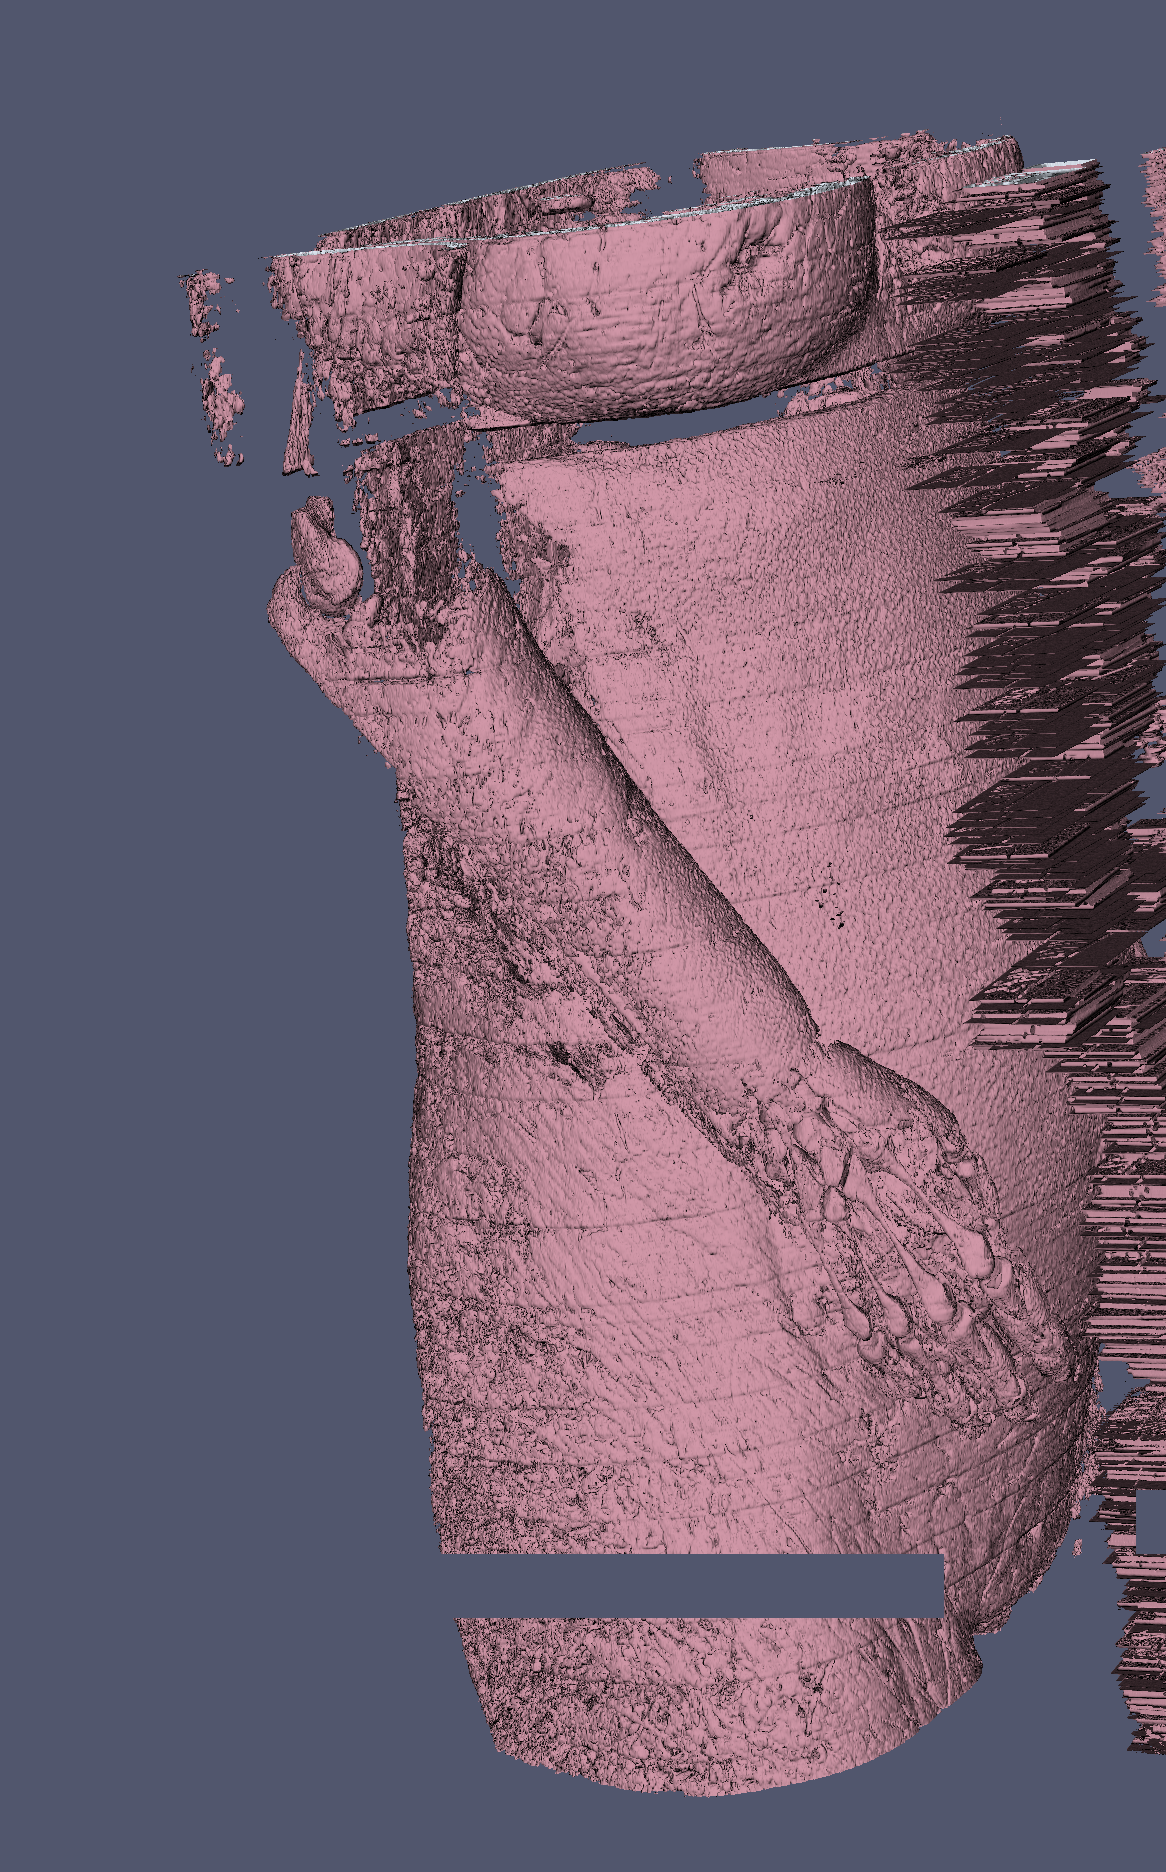
\includegraphics[width=10cm]{Fullbody1.png}
	
	\item[Tool:]
	\hfill \break
		Paraview
	\item[Visual Mappings:]
	
	\begin{itemize}
		\tightlist
		\item[ ]
	\end{itemize}
	
	\begin{itemize}
		\tightlist
		\item
		\textbf{Mapping 1}: 
		\hfill \break
			Between data points 67.972 - 210.121 a pink colour has been assigned, to map to the skin with an opacity of 0.000. However, the opacity has no effect on the Isosurface image. While the values 220.000 to 395.686 have been assigned a white value, as with the data conversion is in composite, the bones are assigned a white colour with an opacity of 0.726.
	\end{itemize}
	
	\begin{itemize}
		\tightlist
		\item
		\textbf{Mapping 2}:
		\hfill \break
			Colour preset was originally cool to warm but has been modified. Colour space LAB has been used with nan opacity to 1. 
	\end{itemize}
	
	\item[Data Conversion:] 
	\hfill \break
		Data spacing used is 1, 1, 4 with a representation of volume. The volume rendering is using OSPRay based with a blend mode of Isosurface. The value range is set to 200.
	
	\item[Unique Observation:]
	\hfill \break
		This scan shows a female's abdomen from the chest to the top of the legs. At data point 127.5, all of the person's skin is shown, but if you assign the range value to data point 200, this is where the visualisation shows the skin but also allows the hand, elbow and forearm bones show through. 
	
\end{description}
